%!TEX root = ../thesis.tex
\section{Evaluation}\label{sec:evaluation}
The evaluation aims to show that the test formalization of \drivebuild{} is general enough to be used with different approaches for implementing test generators and \glspl{ai}.
It also aims to show whether test executions on a single \gls{simnode} on a real machine scale linearly and whether the performance degradation when using \glspl{vm} to host \glspl{simnode} is unbearable.
The evaluation addresses the following main research questions:
% https://library.royalroads.ca/writing-centre/writing/structure/thesis-statements lists a few characteristics RQs should have.
\begin{description}
    \item[RQ1] How comprehensive is the test formalization concerning the support of various kinds of test generators and \glspl{ai}?
        Different approaches for test generators and \glspl{ai} have different requirements when testing them.
        The creation of benchmarks and ratings for comparing test generators and \glspl{ai} to each other introduces even further requirements.
        Thus in order to interact with test generators and \glspl{ai}, to analyze and to offer feedback data the formalization has to fulfill these requirements.
        The evaluation focuses on approaches that \cref{sec:stateOfTheArt} presents to investigate the research question.
    \item[RQ2] How does \drivebuild{} scale over real machines and \glspl{vm}?
        \drivebuild{} is a distributed system and aims to run as many simulations as possible in parallel.
        This research question investigates how many tests a single \gls{simnode} can run without having an influence on the test results, the benefit of utilizing parallelism and whether hosting \glspl{simnode} in \glspl{vm} is a feasible solution to distribute simulations over a cluster.
    \item[RQ3] How supportive is \drivebuild{} for developers in setting up simulations, running tests and collecting data?
        A goal of \drivebuild{} is to lift out testers of tedious and error prone tasks like setting up and managing simulations as well as implementing an interaction between simulations and \glspl{ai}.
        This research question qualitatively evaluates the benefits of using \drivebuild{} compared to manually setting up and executing tests.
        Therefore it compares the effort to understand and use \drivebuild{} to the benefits \drivebuild{} offers.
\end{description}
The evaluation has four subsections.
\Cref{subsec:experimentalSettings} elaborates in which context the evaluation took place and lists all technical specifications which are relevant.
\Cref{subsec:evaluationOfGenerality} describes the test for checking the comprehensiveness of the test formalization and introduces a number of metrics which \drivebuild{} can yield about test generators and \glspl{ai}.
\Cref{subsec:evaluationOfScalability} quantitatively evaluates the scalability of \drivebuild{} concerning the number of simultaneously executed simulations and the number of \glspl{simnode} connected to the \gls{mainapp}.
It also compares the scalability between a \gls{simnode} running on a real machine and \glspl{simnode} hosted on \glspl{vm}.
\Cref{subsec:experienceReport} examines qualitatively the benefits of \drivebuild{}, how supportive it is for testers and the presumably most difficult tasks when using it.
\subsection{Experimental Settings}\label{subsec:experimentalSettings}
\subsubsection{Seminar}
The evaluation took place in the context of the advanced seminar \enquote{Search-based Software Engineering for Testing Autonomous Cars (5846HS)} in summer term 2019 at the University of Passau and had 10 participants which were all either master students or bachelor students in a higher semester.
The students were assigned papers that propose and discuss test generators and approaches for training \glspl{ai}.
As part of the seminar, the students had the task to implement small prototypes of test generators or \glspl{ai} which I will refer to as \enquote{submissions}.
So they have to face problems which are similar to problems real tester have.
The problems include the setup of \beamng{}, the management of simulations and the collection of data which are problems that \drivebuild{} claims to solve.
Hence I targeted the students as users like testers would use \drivebuild{}.
\subsubsection{Submissions}\label{subsubsec:submissions}
\Cref{sec:background} explains all approaches the students used for their submissions.
Three students implemented test generators.
Test generator G1 focuses on generating tests that verify whether \glspl{av} can avoid crashes.
Therefore it uses a predefined list of \num{528} IDs of crash reports referencing the \gls{nhtsa} crash report database which provides these reports as semi-structured \gls{xml}.
G1 utilizes \gls{ac3r}~\cite{ac3r} which generates \beamng{} scenarios.
It parses these \beamng{} scenarios and formalizes them such a way that they can be used with \drivebuild{}.
Test generator G2 aims to generate test scenarios that focus on verifying the lane keeping capabilities of \glspl{av}.
It claims to extend \asfault{}~\cite{asfault} by randomly placing static obstacles all over the area where the road is settled.
Test generator G3 focuses on testing lane keeping capabilities of \glspl{av} as well by applying evolutionary computing to generate a population of interesting roads.
Each call to G3 returns only the first element of the resulting population.
It does not apply any metric to determine a specific element in the population.
Besides the test generators students submitted I created a reference generator G0 which generates random tests using \asfault{}.
The generated tests have one road which is restricted to be placed in an area of \(\SI{100}{\metre}\times\SI{100}{\metre}\).
This road has two lanes and a fixed width of \SI{8}{\metre}.
The initial seed is a random number between \num{0} and \num{10000}.\\
Two of the students implemented \glspl{ai}.
The \gls{ai} A1 is based on a version of deep reinforcement learning which uses \gls{ddpg} and a \gls{vae}.
The student pretrained the \gls{ai} on roads generated by \asfault{}.
\Gls{ai} A2 uses \deepdriving{}.
To pretrain the \gls{ai} the student drove a car manually with \beamng{} on the level which \drivebuild{} uses for its simulations.
Additionally to the \glspl{ai} students implemented I use the \beamng{} \gls{ai} as reference \gls{ai} A0.
This \gls{ai} has perfect knowledge about all roads but does neither recognize any obstacles nor any other participants.
It has an option \enquote{stay on lane} which allows to define a single target waypoint instead of a sequence of consecutive waypoints the \gls{av} has to follow.
The \gls{ai} is able to detect which lanes it has to follow to reach the desired target waypoint.
As a restriction the target waypoint has to be right in the middle of the road otherwise the \beamng{} \gls{ai} does not find a path to it.
\subsubsection{Technical Specifications}
\drivebuild{} is a distributed system and the evaluation utilizes this capability by running the components of \drivebuild{}, test generators, \glspl{ai} and the actual evaluation process across multiple nodes.
\Cref{tab:nodeSpecifications} lists the specifications of all available nodes.
\begin{table}
    \caption{%
        Node specifications --- Lists the specifications for all (virtual) nodes that were used for the evaluation.
    }\label{tab:nodeSpecifications}
    \medskip
    \begin{tabularx}{\textwidth}{X l l l l}
    \toprule
    \bfseries Property     & \bfseries Node~0                   & \bfseries Node~1                     & \bfseries Node~2                     & \bfseries Node~3                       \\
    \midrule
    Hardware/\Glstext{vm}? & \Glstext{vm}                       & Hardware                             & Hardware                             & \Glstext{vm}                           \\
    \Glstext{os}           & Linux Debian                       & \makecell[l]{Windows 10\\Enterprise} & Windows 10 Pro                       & Windows 10 Pro                         \\
    Version                & 10                                 & 1903                                 & 1903                                 & 1903                                   \\
    Build                  & 4.19.0--6                          & 18362.418                            & 18362.418                            & 18362.418                              \\
    Architecture           & 64 bit                             & 64 bit                               & 64 bit                               & 64 bit                                 \\
    \midrule
    \Glstext{cpu}          & \makecell[l]{Intel Xeon\\E5--2630} & \makecell[l]{Intel Core\\i7--7700K}  & \makecell[l]{Intel Core\\i7--7700HQ} & \makecell[l]{Intel Xeon\\E3--12xx v2}  \\
    Clock Rate             & \SI{2.4}{\GHz}                     & \SI{4.2}{\GHz}                       & \SI{2.8}{\GHz}                       & \SI{3}{\GHz}                           \\
    Logical Cores          & \num{8}                            & \num{8}                              & \num{8}                              & \num{2}                                \\
    \midrule
    \Glstext{ram}          & \SI{8}{GB}                         & \SI{16}{GB}                          & \SI{16}{GB}                          & \SI{16}{GB}                            \\
    \midrule
    \Glstext{gpu}          & \textit{Not used}                  & \makecell[l]{GeForce\\GTX 1080}      & \makecell[l]{GeForce\\GTX 1070}      & \makecell[l]{GeForce GTX\\Titan Black} \\
    Driver Version         & \textit{Not used}                  & 436.48                               & 436.48                               & 436.30                                 \\
    \bottomrule
\end{tabularx}

\end{table}
During the evaluation node~0 hosts one instance of the \gls{mainapp} which is accessible from all the other nodes and node~1 runs all the submitted test generators, \glspl{ai} and the \submissiontester{} which encapsulates the execution of the submissions, their interaction with \drivebuild{}, the preprocessing of tests and the collection of data for the evaluation.
Node~2 and one or multiple instances of node~3 may run instances of \glspl{simnode} depending on the current test setup.
Each active instance of these nodes hosts exactly one \gls{simnode}.

\subsection{Evaluation of Generality}\label{subsec:evaluationOfGenerality}
The evaluation of the generality of the test formalization considers two main aspects.
The first aspect is the feature coverage that determines which features of \drivebuild{} were used during the evaluation and which submissions used them.
The second aspect examines on the one hand which metrics the submissions require to operate and whether \drivebuild{} provides them and on the other hand which further metrics \drivebuild{} offers to create detailed analysis about the submissions.
All time measurements in any evaluation use real time over simulation time since measuring real time is at many points easier than measuring simulation time.
Further real time considers in contrast to the simulation time the time test generators require to generate new tests as well as the time \glspl{ai} need to calculate control commands.
\subsubsection{Challenge Test}
In order to investigate these aspects the challenge test runs the submitted \glspl{ai} against the submitted test generators.
In terms of the challenge test a combination of a test generator and an \gls{ai} is called a \enquote{match} and has a fixed time budget.
One execution of the challenge test lets each \gls{ai} compete against each test generator.
Each match repeats the following steps again and again until the given time budget is used.
First, the selected test generator generates a test.
In case the generator succeeded the \submissiontester{} checks multiple validity constraints which ensure that the test can be executed and that it can be compared with generated tests of other test generators.
A test is only valid if it defines at least one participant with the name \enquote{ego}, defines at least one road and the generated citeria (\Glstext{dbc}) references the generated environment (\Glstext{dbe}).
If the \submissiontester{} considers the test valid it further modifies the test to ensure comparability with other tests and compatibility with the \gls{ai} assigned to the match:
It enforces a failure criterion which makes the test fail if any participants is off-road or damaged.
It also forces the \gls{av} \enquote{ego} to be in movement mode \mmautonomous{} during the whole simulation and any other participants to be in movement mode \mmtraining{} to make sure it can collect data about all participants.
To enable the assigned \gls{ai} to operate properly the \submissiontester{} adds data requests to the test for all monitoring data the \gls{ai} requires.
For the analysis of the submissions it adds even more data requests to every participant which store the heading angle as well as the position of the participant.
In case of A0 the \submissiontester{} has to define a target position for the \gls{ai}.
\Cref{subsec:targetPositionDetermination} describes the process of finding an appropriate target position in detail.\\
The \submissiontester{} submits the preprocessed test to \drivebuild{}.
If \drivebuild{} accepts the test the \submissiontester{} creates one instance of the assigned \gls{ai} and connects it to the \gls{av} with ID \enquote{ego}.
I execute the challenge test in different configurations.
An execution defines the time budget for matches either with \SI{10}{\minute} or \SI{30}{\minute} and enforces road markings or no road markings.
Additionally I repeat each execution once which results in a total of \num{8} executions.
At the end this yielded a total number of \num{1208} generated tests.
\subsubsection{Interfaces for Challenge Test}
To allow the \submissiontester{} to work with all submissions homogeneously they have to implement predefined interfaces.
A test generator has to provide a class with a method having the signature given in \cref{fig:testGeneratorStub}.
\begin{figure}
    \captionsetup{type=listing}
    \inputminted{python}{code/testGeneratorStub.py}
    \medskip
    \caption{%
        Test generator stub --- Describes the stub for the implementation of a test generator.
    }\label{fig:testGeneratorStub}
\end{figure}
The method \code{getTest()} does not accept any input and returns a tuple with two paths where the first points to a \gls{dbe} file and the second to a \gls{dbc} file which references the \gls{dbe} file. % chktex 36
The method may return \code{None} if the generator is not able to generate more tests.\\
An implementation of an \gls{ai} has to implement the interface \cref{fig:aiStub} shows.
\begin{figure}
    \captionsetup{type=listing}
    \inputminted{python}{code/aiStub.py}
    \medskip
    \caption{%
        \Glstext{ai} stub --- Shows the scheme of the implementation of \glspl{ai} required for the evaluation and uses the client scheme of \cref{fig:clientScheme}.
    }\label{fig:aiStub}
\end{figure}
The constructor of the \gls{ai} accepts an instance representing the connection to \drivebuild{}.
This connection provides methods for the \gls{ai} to request data and control \glspl{av}.
The method \code{add\_data\_requests(\ldots)} adds data requests (see \cref{fig:exampleAIDataRequests}) which the \gls{ai} requires for operation to the declarations of \glspl{av}. % chktex 36
Therefore it accepts the \gls{xml} tag to which the data requests have to be added to and the ID of the \gls{av} for which the data requests are declared.
This ID should be used to create unique IDs for the declared data requests.
The method \code{start(\ldots)} follows the client scheme (see \cref{fig:clientScheme}) which implements the interaction between an \gls{ai} and \drivebuild{}. % chktex 36
It accepts the ID of the simulation which simulates the \gls{av} to control, the ID of \gls{av} itself and a callback method which gathers runtime data about the simulation for the evaluation afterwards.
\subsubsection{Feature Coverage}
The feature coverage indicates which features of \drivebuild{} were used during the evaluation and thus it suggests which features are somewhat tested and presumably work as they are expected.
\Cref{tab:featureCoverage} summarises the most basic features \drivebuild{} provides and which submissions use them.
\begin{table}
    \centering
    \caption{%
        Feature coverage --- Summarizes which features are used by the submissions and the evaluation.
        If a cell contains check mark a submission or the evaluation uses the feature intentionally.
        If a cell contains a tilde the feature is used only sometimes and the submission is not explicitly designed to use it.
    }\label{tab:featureCoverage}
    \medskip
    %!TEX root = ../thesis.tex
\begin{tabularx}{.6\linewidth}{X c c c c}
    \toprule
    \bfseries Feature                          & \bfseries G0 & \bfseries G1 & \bfseries G2 & \bfseries G3         \\
    \midrule
    \multicolumn{5}{c}{Scenario Elements}                                                                          \\
    Multiple participants                      &              & \checkmark{} &              &                      \\
    Obstacles                                  &              &              & \checkmark{} &                      \\
    Multiple roads                             &              & \checkmark{} &              &                      \\
    Intersections                              & \~{}         & \checkmark{} & \~{}         & \~{}                 \\
    \midrule
    \multicolumn{5}{c}{Test Configuration}                                                                         \\
    Road markings                              & \checkmark{} & \checkmark{} & \checkmark{} & \checkmark{}         \\
    Speed limits                               &              &              &              &                      \\
    Target speeds                              &              &              &              &                      \\
    \midrule
                                               & \bfseries A0 & \bfseries A1 & \bfseries A2 & \bfseries Evaluation \\
    \midrule
    \multicolumn{5}{c}{Data Requests}                                                                              \\
    Camera images                              &              & \checkmark{} & \checkmark{} &                      \\
    Speed                                      &              &              & \checkmark{} &                      \\
    Position                                   &              &              &              & \checkmark{}         \\
    Bounding box                               &              &              &              & \checkmark{}         \\
    \midrule
    \multicolumn{5}{c}{Criteria}                                                                                   \\
    Damage detection                           &              &              &              & \checkmark{}         \\
    Off-road detection                         &              &              &              & \checkmark{}         \\
    Goal area detection                        &              &              &              & \checkmark{}         \\
    \Glstext{vc}                               &              &              &              &                      \\
    \bottomrule
\end{tabularx}

\end{table}
The submissions use only a very restricted subset of the features that \drivebuild{} offers.
There is only one test generator which declares obstacles.
There is also only one test generator which defines more than a single participant on a single road and which intentionally creates intersections.
That the test generators use the road markings feature results from the fact that the configuration of the challenge test enforces them.
The \glspl{ai} rely on camera images and one \gls{ai} additionally relies on the current speed of an \gls{av}.
The evaluation part of the table includes features to evaluate the challenge test as well as the test criteria.
The evaluation uses only features which are related to check and analyse the lane keeping capabilities of \glspl{ai}.
The evaluation does not declare any criteria that use \glsfirstplural{vc}.\\
As a conclusion the small set of used features is sufficient to support all submissions and to create metrics to analyze them.
\drivebuild{} offers many more features which are not listed in \cref{tab:featureCoverage}.
Since neither the submissions nor the evaluation use them their investigation is subject of future.
\subsubsection{Efficiency of Test Generators}
The efficiency of test generators is a metric to identify how many valid tests a generator can produce in a given time interval.
\Cref{fig:exectionTimes} visualizes the distribution of the duration of the executed tests.
\begin{figure}
    \includesvg[width=\textwidth]{diagrams/diagram17a.svg}
    \medskip
    \caption{%
        Execution times --- Visualizes the durations of executed simulations and their standard deviation.
        The execution time includes generation of a test, upload to \drivebuild{}, start of a simulator instance, running the test until it finishes.
        This diagram shows only execution times of tests which did not encounter a timeout.
    }\label{fig:exectionTimes}
\end{figure}
The efficiency \(e\) of the test generators is \num{1} divided by the average time per test execution \(t_{avg}\) (see \cref{eq:efficiency}).
\begin{equation}
    \label{eq:efficiency}
    e = 1 / t_{avg}
\end{equation}
The average execution time \(t_{avg}\) for G0 is \SI{1.75}{\minute}, for G1 \SI{0.70}{\minute}, for G2 \SI{0.28}{\minute} and for G3 \SI{0.60}{\minute}.
G2 is by far the most efficient test generator.
G1 and G3 have a similar efficiency despite the fact that G1 uses \gls{ac3r} which focuses on generating very compact test scenarios and should result in short execution times whereas G3 uses a \gls{ga} to evolve tracks.
G0 is clearly the least efficient test generator although G2 claims to use \asfault{} the same way.
\Cref{fig:numberOfTests} groups the generated tests by test generator and compares the number of generated tests based on the available time budget of the challenge test execution.
\begin{figure}
    \includesvg[width=\textwidth]{diagrams/diagram16a.svg}
    \medskip
    \caption{%
        Number of generated tests --- Shows how many valid and invalid tests each of the test generators generated in total during the challenge test.
        The diagram groups them by the time budget available in a round.
        It also shows their standard deviation.
    }\label{fig:numberOfTests}
\end{figure}
When comparing the number of generated tests in executions with different time budgets the number of generated tests within \SI{30}{\minute} is about three times as high as within \SI{10}{\minute}.
This suggests that the efficiency of the test generators does not decrease the longer they run although some of them should rely on feedback data.
A validation of this statement requires many more executions of the challenge which is not done during this thesis.
\subsubsection{Complexity of Test Cases}
Metrics about the complexity of generated tests allow to estimate how difficult it is for an \gls{av} to succeed a test.
Depending on which properties of an \gls{av} have to be tested different aspects of complexity are considered.
Since most of the submitted test generators test lane keeping capabilities the evaluation investigates the complexity of the generated environments and how far \glspl{av} traveled.
For the metrics I use amongst others the number of scenario elements \ie{} participants, obstacles and roads plus the complexity of the curvature and the length of the generated roads.\\
\Cref{fig:numElements} visualizes the number of scenario elements.
\begin{figure}
    \includesvg[width=\textwidth]{diagrams/diagram9a.svg}
    \includesvg[width=\textwidth]{diagrams/diagram11a.svg}
    \includesvg[width=\textwidth]{diagrams/diagram10a.svg}
    \medskip
    \caption{%
        Number of scenario elements --- Shows which types of scenario elements like participants, roads and obstacles generated tests included and how many.
    }\label{fig:numElements}
\end{figure}
Every test generated by G0, G2 or G3 declares exactly one road and one participant.
In contrast to any other generator G1 often defines two roads and one participant on each road.
This is due to the fact that G1 uses crash reports to generate test cases and the crash reports that the underlying database provides most commonly involve two participants and often intersections.
G2 is the only generator that adds static obstacles to its tests since the student who implemented it had the explicitly the task to generate tests with obstacles.\\
\Cref{fig:roadLengths} shows the distribution of the lengths of the generated roads.
\begin{figure}
    \includesvg[width=\textwidth]{diagrams/diagram8a.svg}
    \medskip
    \caption{%
        Road lengths --- Visualizes the lengths of the generated roads grouped by test generator.
        The longer a road is the potentially more complex its curvature might be.
    }\label{fig:roadLengths}
\end{figure}
The shorter generated roads are the less potential they have to have a complex and diverse curvature.
The longer the generated roads are the longer the execution of a test takes for an \gls{av} to succeed.
G0, G2 and G3 generate roads of very similar length but G3 has a little less variety in their length.
G1 generates much shorter roads which is a result of \gls{ac3r} which aims to generate very compact test scenarios.
This indicates that G1 does not define complex roads.\\
\Cref{fig:numRoadSegments} depicts the distribution of the number of segments that define each generated road.
\begin{figure}
    \includesvg[width=\textwidth]{diagrams/diagram7a.svg}
    \medskip
    \caption{%
        Number of road segments --- Depicts the number of road segments that were used for any road generated during the challenge test.
        It groups them by test generator.
    }\label{fig:numRoadSegments}
\end{figure}
The lower the number of road segments the lower is the potential of the road to have a complex and diverse curvature.
The fewer road segments define a road and the longer the road is the more likely it is that the generated curvature differs from what the test generator intended since it relies more on the interpolation done by \drivebuild{}.
Every road generated by G1 has a low number of segments which fits well with the goal of \gls{ac3r} to create very compact tests.
G3 uses a constant number of road segments.
The initial population is a set of randomly placed positions which define the segments of a road.
Based on this population the \gls{ga} which G3 applies evolves tracks by repositioning the segments.
G2 uses a constant number of road segments as well but the number of segments is much lower.
Since the roads are much longer compared to roads of other generators it is likely that they have many long and only slightly winding sections and may not have a very diverse curvature.
The constant number of road segments further indicates that the implementation of G2 does not use \asfault{} to generate random roads as it was supposed to do.
This becomes especially clear when compared to G0.
The number of road segments generated by G0 has a much higher variety.
Combining this observation with the fact that the length of the generated roads has a variety similar to G2 and G3 indicates that the generated roads may have in some cases more linear and in others more winding sections.\\
\Cref{fig:roadVisualization} supports these observations.
\begin{figure}
    \centering
    %!TEX root = ../thesis.tex
\setlength{\fboxsep}{0pt}
\begin{subfigure}[c]{.49\linewidth}
    \fbox{
        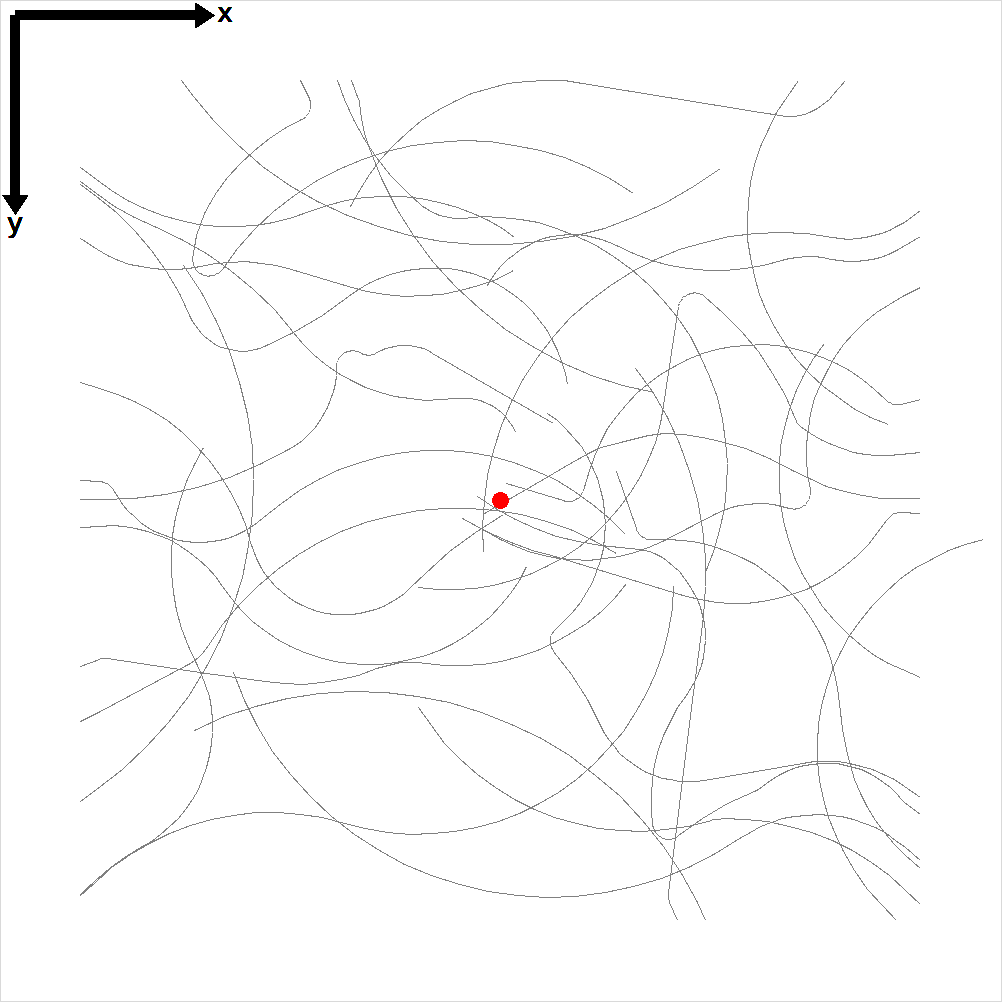
\includegraphics[width=.96\linewidth]{diagrams/roadVisualization_G0.png}
    }
    \subcaption{%
        Roads generated by G0
    }
\end{subfigure}
\begin{subfigure}[c]{.49\linewidth}
    \fbox{
        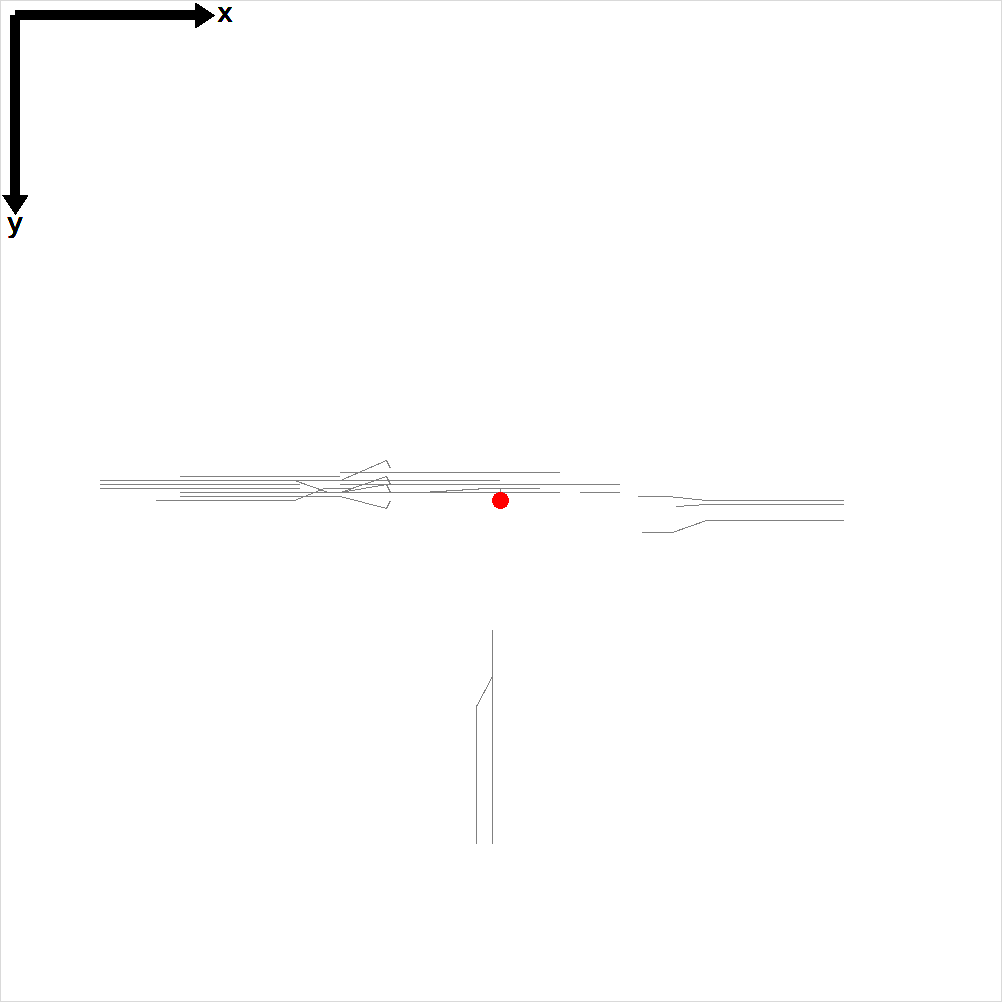
\includegraphics[width=.96\linewidth]{diagrams/roadVisualization_G1.png}
    }
    \subcaption{%
        Roads generated by G1
    }
\end{subfigure}
\begin{subfigure}[c]{.49\linewidth}
    \fbox{
        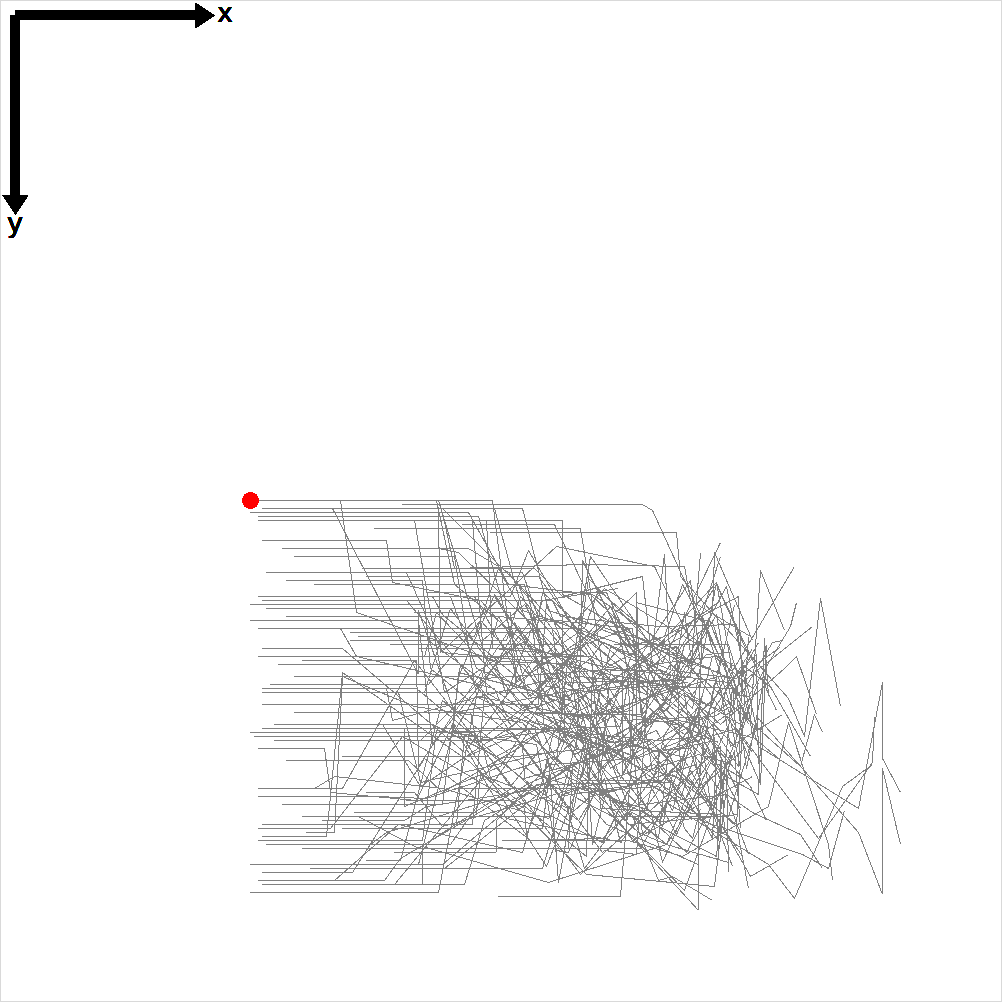
\includegraphics[width=.96\linewidth]{diagrams/roadVisualization_G2.png}
    }
    \subcaption{%
        Roads generated by G2
    }\label{subfig:roadVisualizationG2}
\end{subfigure}
\begin{subfigure}[c]{.49\linewidth}
    \fbox{
        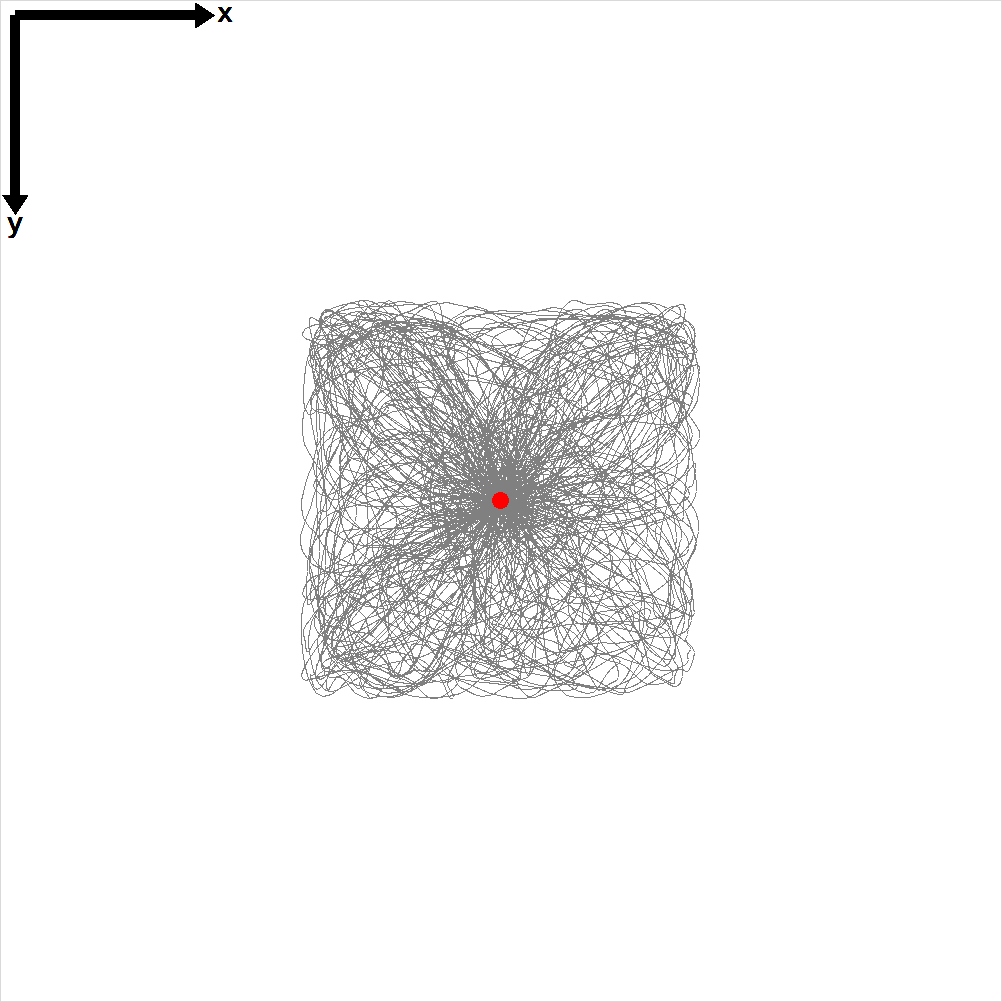
\includegraphics[width=.96\linewidth]{diagrams/roadVisualization_G3.png}
    }
    \subcaption{%
        Roads generated by G3
    }
\end{subfigure}

    \medskip
    \caption{%
        Visualization of roads --- Visualizes the segments of all generated roads.
        Each picture covers all points where \(-250<x<250\) and \(-250<y<250\) except for \cref{subfig:roadVisualizationG2} which is shifted to cover all points with \(-125<x<375\).
        The red point marks the origin.
        The points are connected with straight lines instead of interpolating them as they are when starting a simulation.
    }\label{fig:roadVisualization}
\end{figure}
Further it shows that G1 and G2 restrict the segments of the generated roads to be placed in an area of a size \(\SI{200}{\metre}\times\SI{200}{\metre}\) whereas G3 only uses an area of size \(\SI{100}{\metre}\times\SI{100}{\metre}\).
In comparison G0 uses a larger area and distributes its lanes over the available area.\\
To get an impression about the variety of curvatures of the generated roads \cref{fig:roadCurvatureVisualization} shows the roads rotated and translated such a way that the first road center point is in the origin and the second is right below of it.
\begin{figure}
    \centering
    %!TEX root = ../thesis.tex
\setlength{\fboxsep}{0pt}
\begin{subfigure}[c]{.49\linewidth}
    \fbox{
        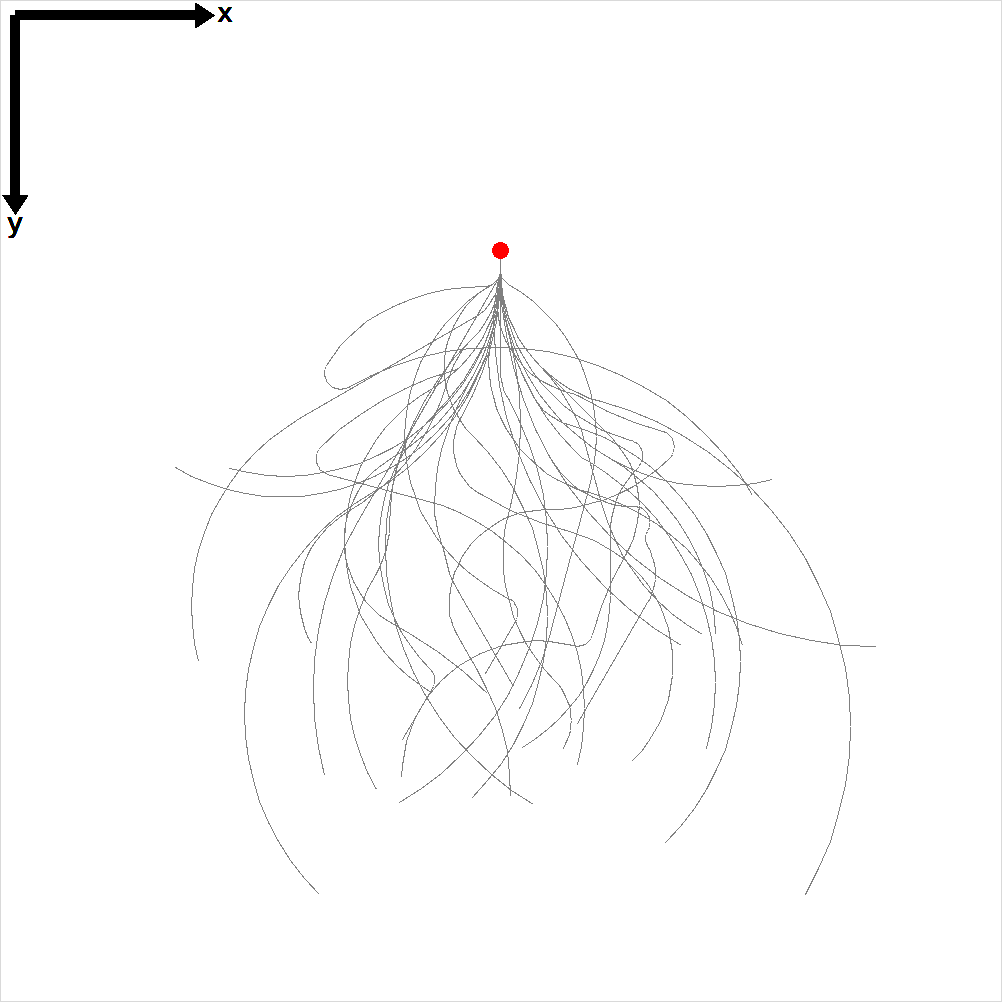
\includegraphics[width=.96\linewidth]{diagrams/roadVisualization_G0_translated.png}
    }
    \subcaption{%
        Curvature of roads generated by G0
    }
\end{subfigure}
\begin{subfigure}[c]{.49\linewidth}
    \fbox{
        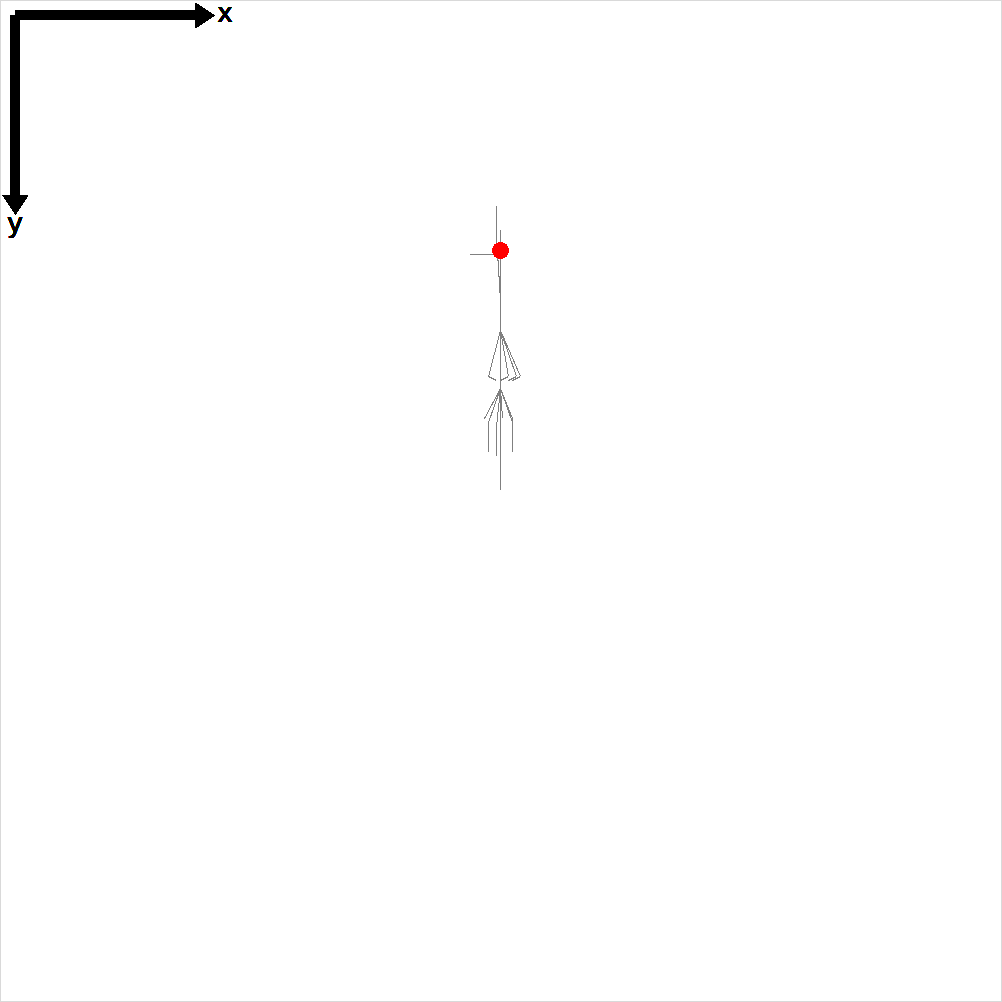
\includegraphics[width=.96\linewidth]{diagrams/roadVisualization_G1_translated.png}
    }
    \subcaption{%
        Curvature of roads generated by G1
    }
\end{subfigure}
\begin{subfigure}[c]{.49\linewidth}
    \fbox{
        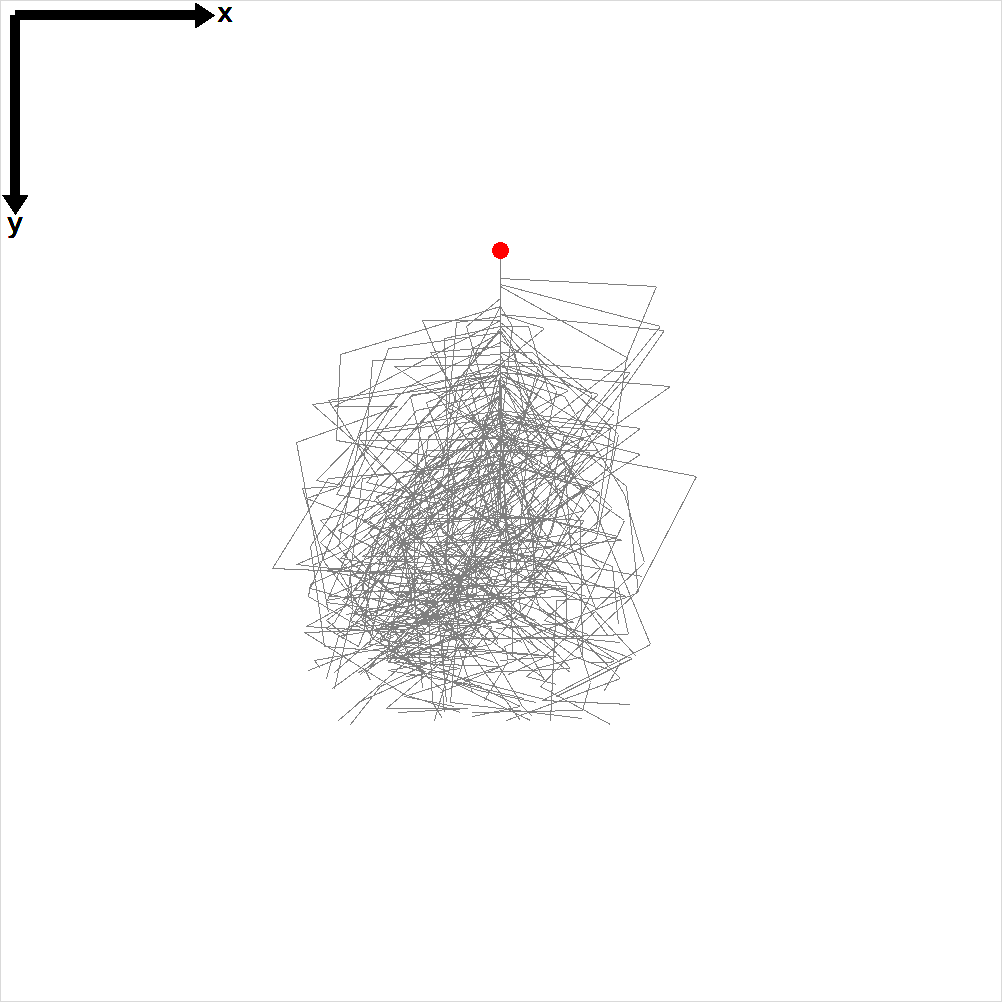
\includegraphics[width=.96\linewidth]{diagrams/roadVisualization_G2_translated.png}
    }
    \subcaption{%
        Curvature of roads generated by G2
    }
\end{subfigure}
\begin{subfigure}[c]{.49\linewidth}
    \fbox{
        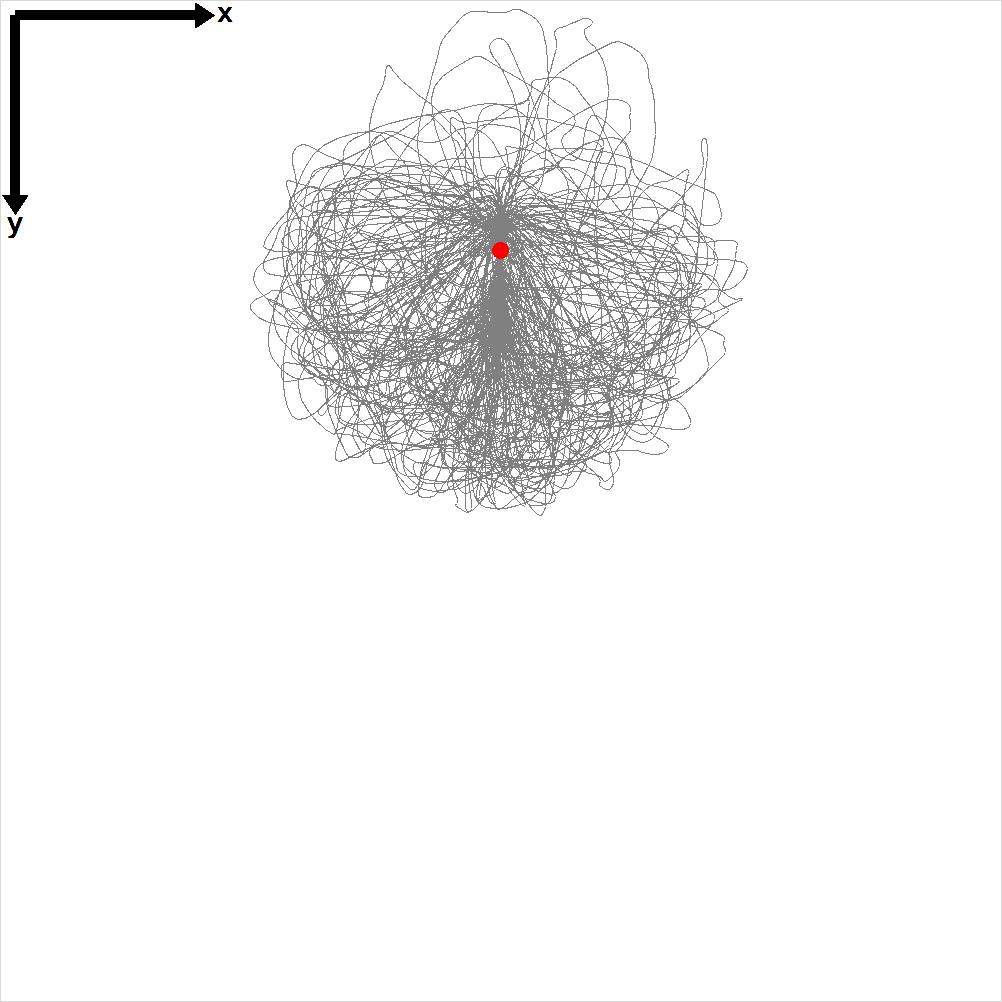
\includegraphics[width=.96\linewidth]{diagrams/roadVisualization_G3_translated.png}
    }
    \subcaption{%
        Curvature of roads generated by G3
    }
\end{subfigure}

    \medskip
    \caption{%
        Visualization of road curvatures --- Visualizes the segments of all generated roads but equally rotated based on the first two road segments and translated to start at the origin.
        Each picture covers all points where \(-250<x<250\) and \(-125<y<375\).
        The red point marks the origin.
    }\label{fig:roadCurvatureVisualization}
\end{figure}
The roads generated by G0 consist mainly of one or two big curves and often face in a similar direction.
Only occasionally a road has multiple curves that head in different directions and it rarely has sharp turns or long straight sections.
G1 generates solely almost short and straight roads as expected from \gls{ac3r}.
The center points of the roads generated by G2 seem to be uniformly and randomly distributed over a predefined area which contradicts with its claim to use \asfault{} for the generation.
G3 generates highly diverse and complex roads with many curves having different directions and sizes.
The generated roads may even revolve the initial position which makes the roads interesting on an intuitive level.
To estimate how interesting the generated roads are future work may use quantitative metrics~\cite{generationForRacingGames} to further investigate the generated roads.\\
\Cref{fig:traveledDistancesVisualization} visualizes how far \glspl{av} traveled on generated roads.
\begin{figure}
    \centering
    %!TEX root = ../thesis.tex
\setlength{\fboxsep}{0pt}
\begin{subfigure}[c]{.49\linewidth}
    \fbox{
        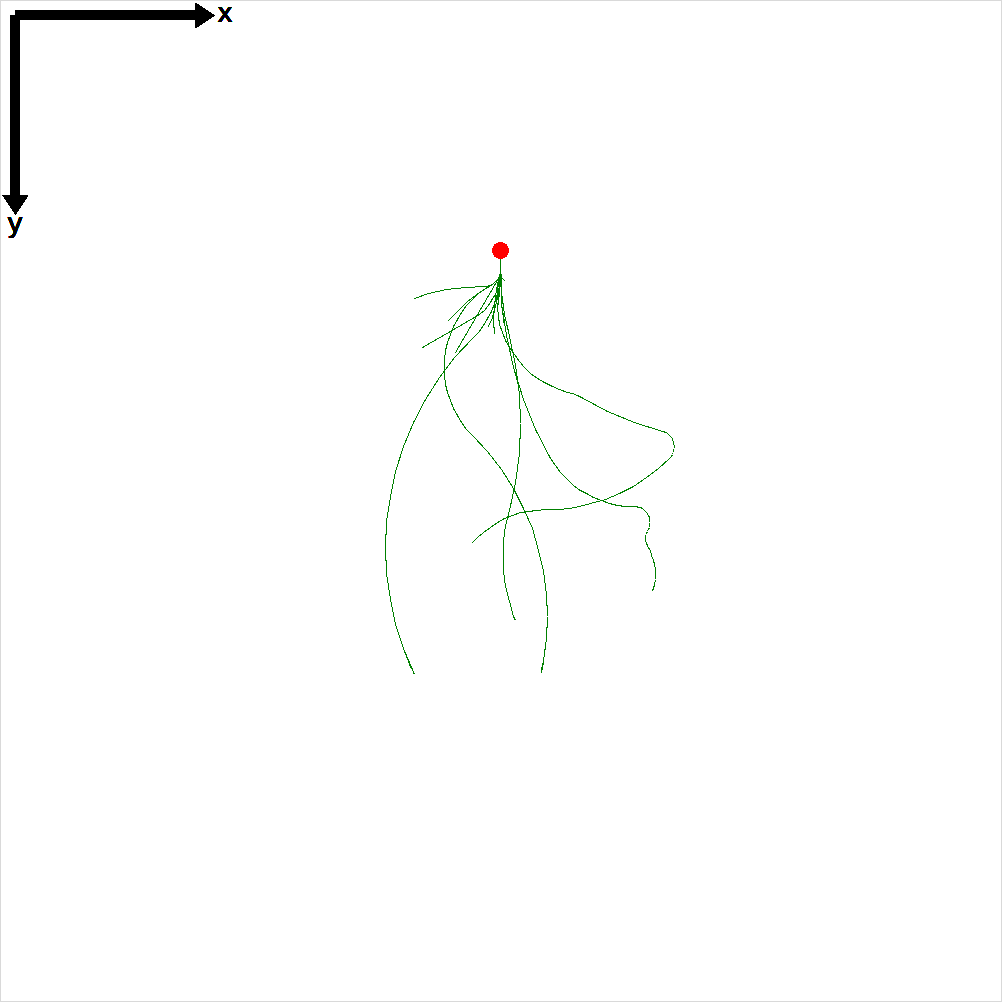
\includegraphics[width=.96\linewidth]{diagrams/roadVisualization_G0_traveled.png}
    }
    \subcaption{%
        Traveled distances on roads generated by G0
    }
\end{subfigure}
\begin{subfigure}[c]{.49\linewidth}
    \fbox{
        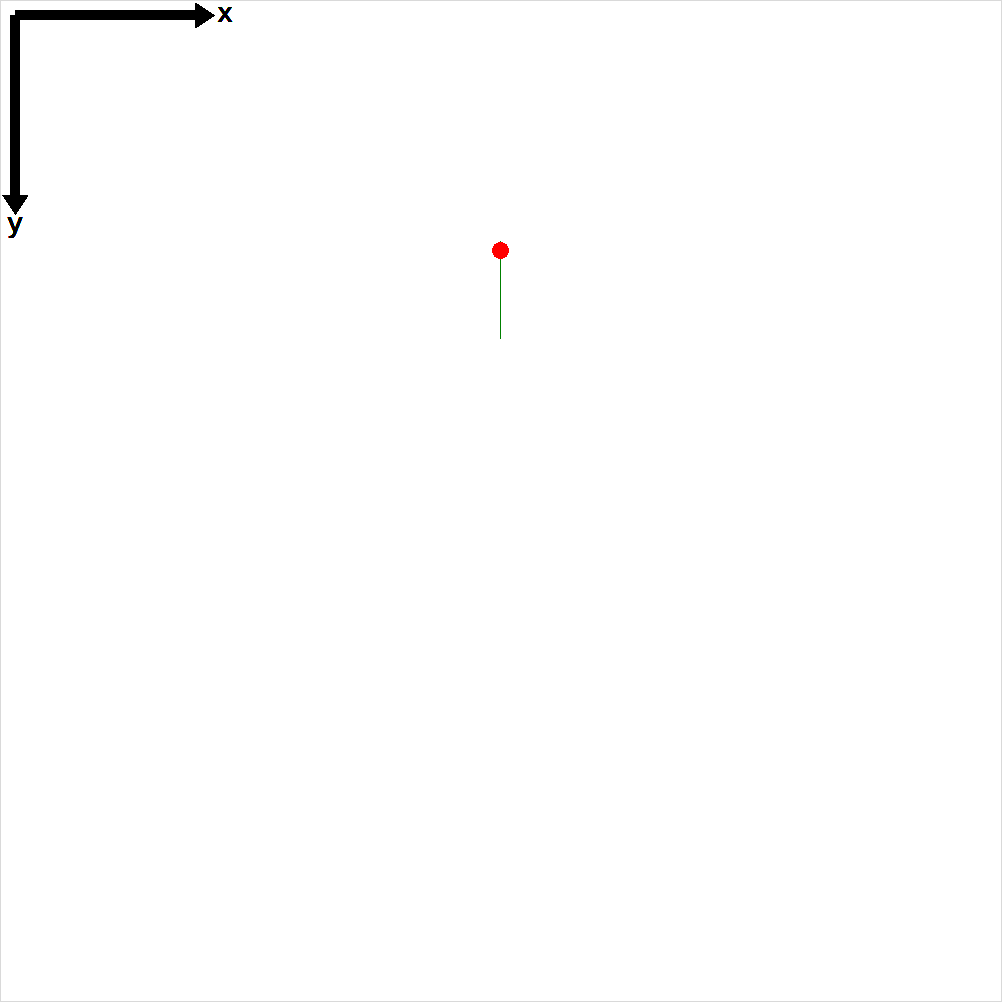
\includegraphics[width=.96\linewidth]{diagrams/roadVisualization_G1_traveled.png}
    }
    \subcaption{%
        Traveled distances on roads generated by G1
    }
\end{subfigure}
\begin{subfigure}[c]{.49\linewidth}
    \fbox{
        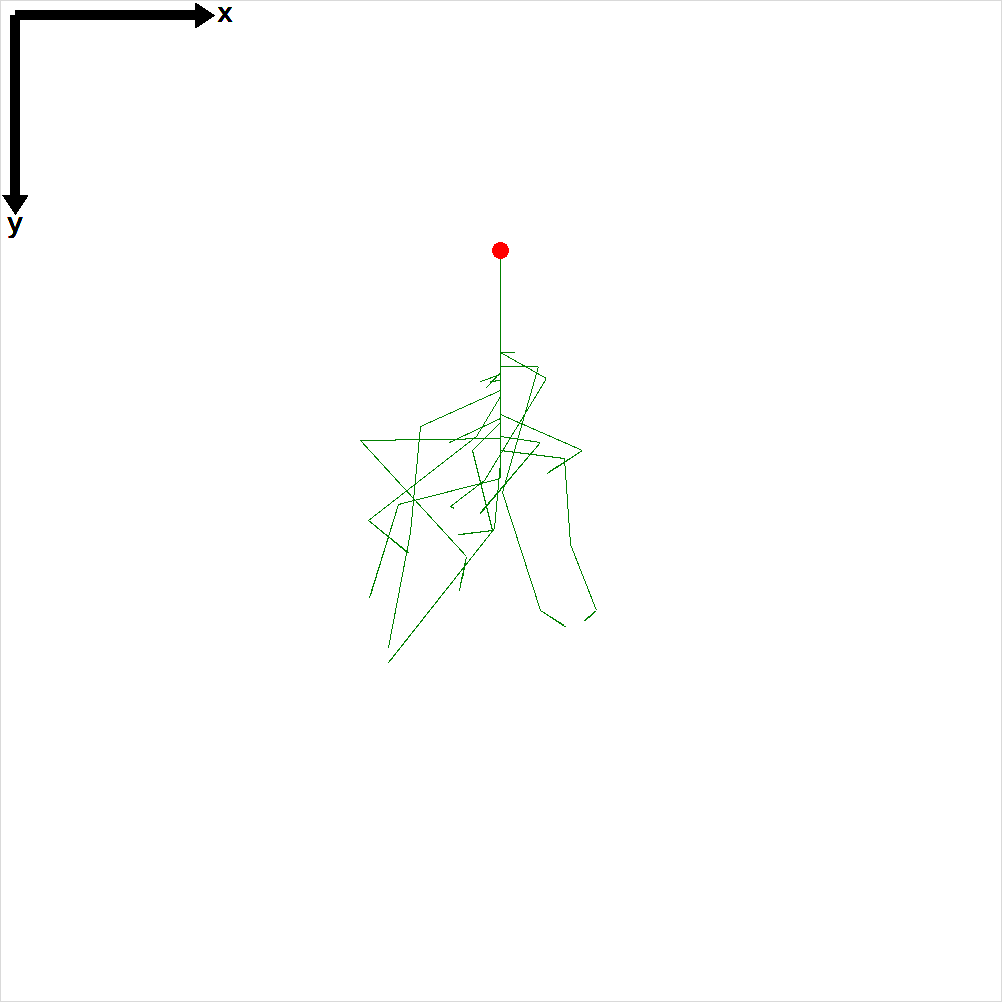
\includegraphics[width=.96\linewidth]{diagrams/roadVisualization_G2_traveled.png}
    }
    \subcaption{%
        Traveled distances on roads generated by G2
    }
\end{subfigure}
\begin{subfigure}[c]{.49\linewidth}
    \fbox{
        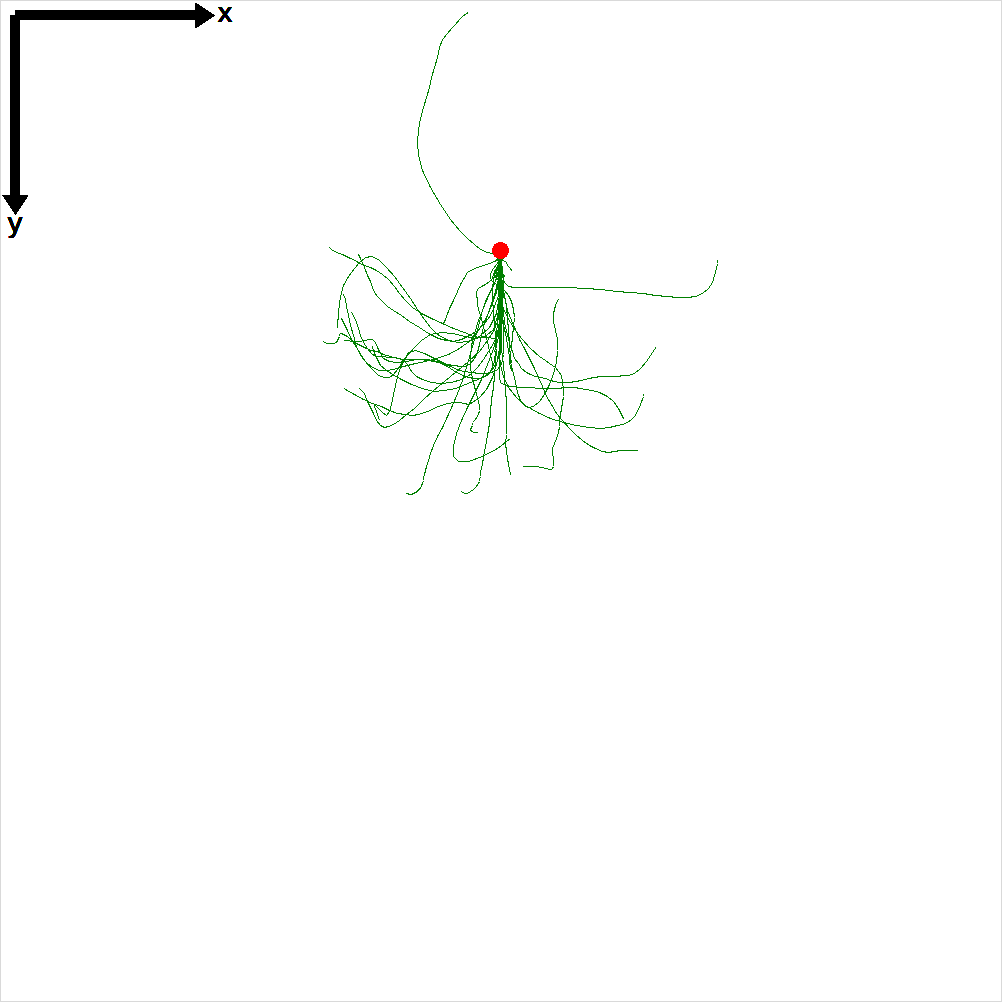
\includegraphics[width=.96\linewidth]{diagrams/roadVisualization_G3_traveled.png}
    }
    \subcaption{%
        Traveled distances on roads generated by G3
    }
\end{subfigure}

    \medskip
    \caption{%
        Visualization of traveled distances --- Visualizes the segments of all roads in \cref{fig:roadCurvatureVisualization} but depicts only the actually traveled segments.
        Each picture covers all points where \(-250<x<250\) and \(-125<y<375\).
        The red point marks the origin.
    }\label{fig:traveledDistancesVisualization}
\end{figure}
Comparing \cref{fig:traveledDistancesVisualization} with \cref{fig:roadCurvatureVisualization} shows that the ratio of the distance \glspl{av} under test traveled to the length of the roads is low.
This confirms that either the \glspl{ai} have no good lane keeping capabilities except for A0 which has perfect knowledge about the lanes or the test generators are very effective in finding bugs in the lane keeping capabilities of \glspl{ai}.
\subsubsection{Effectiveness of Test Generators}
The effectiveness estimates how effectively a test generator can find bugs in \glspl{ai}.
The effectiveness of test generators is computed by dividing the number of failed tests through the sum of failed and successful tests.
The \num{8} executions of the challenge test yielded in total \num{1208} generated tests where \num{1114} were valid and could be executed.
\Cref{fig:numTestsPerGenerator, fig:numTestsPerAI} show all test results and group them by either the test generator or the \gls{ai}.
\begin{figure}
    \includesvg[width=\textwidth]{diagrams/diagram12a.svg}
    \medskip
    \caption{%
        Test results --- Depicts the number of generated tests and groups them by test generator.
        It further distinguishes the number of generated tests based on their test result where \code{ERRORED} and \code{NOT MOVING} are no actual test results but denote that the test generator failed to generate a test or the connected \gls{ai} did not move respectively.
    }\label{fig:numTestsPerGenerator}
\end{figure}
\begin{figure}
    \includesvg[width=\textwidth]{diagrams/diagram12c.svg}
    \medskip
    \caption{%
        Test results --- Divides the executed tests by their result and groups them by the connected \gls{ai}.
        The test results \code{NOT MOVING} and \code{ERRORED} are no actual test results but denote that an \gls{ai} did not move or its implementation threw an error.
    }\label{fig:numTestsPerAI}
\end{figure}
The computation of the effectiveness considers only successful and failed tests but there are more tests.
According to \cref{fig:numTestsPerGenerator} G0 and G1 \gls{av} did not move in some tests.
An \gls{av} is considered as non moving if it does not move more than \SI{5}{\metre} within the first \SI{60}{\second} of the simulation.
These two values are chosen based on a sophisticated guess considering the startup time of \beamng{} and the possible computation overhead of the connected \gls{ai}.
Since according to \cref{fig:numTestsPerAI} the only \gls{ai} that did not move in some tests cases is A0 it is very likely that G0 and G1 did not always define goal positions that fulfill all restrictions inherited by the \beamng{} \gls{ai}.
Additionally many generations of G1 resulted in an error.
According to the log of the challenge executions errors occur because the download of a police report fails, \gls{ac3r} throws an error or \gls{ac3r} is not able to translate the police report into a comprehensive simulation.
In addition many tests result in a timeout which means that a test does neither fail nor succeed within a predefined time.
This can happen if the connected \gls{ai} does not respond \ie{} continue with the execution of the client scheme or the success criterion is either infeasible or the \gls{ai} requires more knowledge about the scenario to fulfill it \eg{} a goal area which is behind but not in front of the \gls{av}.
This timeout consideration applies also for G3.\\
\Cref{tab:effectivenessGenerators} lists how many of the executed tests succeeded and failed per test generator as well as the resulting effectiveness.
\begin{table}
    \centering
    \caption{%
        Test generator effectiveness --- Displays the calculation of the effectiveness of the test generators.
        Higher values indicate higher effectiveness.
    }\label{tab:effectivenessGenerators}
    \medskip
    \begin{tabularx}{.5\linewidth}{X c c c c}
    \toprule
    \bfseries Property & \bfseries G0 & \bfseries G1 & \bfseries G2 & \bfseries G3 \\
    \midrule
    \#Failed      & \num{161}  & \num{117}  & \num{200}  & \num{198}  \\
    \#Succeeded   & \num{32}   & \num{36}   & \num{229}  & \num{73}   \\
    Sum           & \num{193}  & \num{153}  & \num{429}  & \num{271}  \\
    Effectiveness & \num{0.83} & \num{0.76} & \num{0.47} & \num{0.73} \\
    \bottomrule
\end{tabularx}

\end{table}
Compared to the other generators G2 is less effective in generating tests that trigger faulty behavior of \glspl{ai} although it should be very similar to G0.
Both generate always exactly one participant which drives on a single road and both claim to use \asfault{} for generating roads.
G2 has in contrast to G0 very small roads and additionally adds obstacles to its test scenarios (see \cref{fig:numElements}).
So one would expect G2 to be more effective than G0 since it should be more likely that an \gls{av} goes off-road or crash into an obstacle. 
This is clearly not the case.
G0, G1 and G3 have a high effectiveness which mainly results from the bad lane capabilities of the \glspl{ai} that the short traveled distances (see \cref{fig:traveledDistancesVisualization}) suggest.\\
According to \cref{fig:numElements} G1 is the only generator that adds more than one participant and one road.
Since the \glspl{ai} focus on lane keeping and not on crash avoidance the test generators reveals many bugs and therefore it has a high effectiveness.
\Cref{fig:goalRegionSizes} shows the area sizes of the goal regions (in \si{\metre^2}) the test generators defined for the \gls{av} under test to reach.
\begin{figure}
    \includesvg[width=\textwidth]{diagrams/diagram13a.svg}
    \medskip
    \caption{%
        Goal area sizes --- Shows the sizes of generated goal areas that vehicles have to reach in order to succeed a test.
        It only considers valid goal definitions of goal regions.
    }\label{fig:goalRegionSizes}
\end{figure}
The area of the goal regions G0 generates is constant.
To define the goal region in a test G0 selects the road center point of the last segment of the generated road and specifies at this point a goal position having a tolerance radius identical to the width of the road.
Since the width was fixed during the challenge test the size of the resulting goal regions is constant.
In a similar way G3 chooses one of the road center points and defines the goal region by a square with a fixed edge length of \SI{20}{\metre} around the point.
So the size of the resulting goal areas is constant as well.
G1 generates the smallest goal areas which results from the fact that the generated tests are very compact and do not require big goal areas.
G2 generates vastly bigger goal areas which are likely to contain almost the whole environment.
A look into the implementation of G2 reveals that it uses the first and the last two road center points to create a huge triangle which then defines the goal region of a test.
Hence often an \gls{av} almost immediately succeeds a test without driving at all which leads to the low effectiveness of G2.
\Cref{fig:executionTimesAIs} depicts for how long \glspl{ai} drove in simulations of generated tests and supports this observation.
\begin{figure}
    \includesvg[width=\textwidth]{diagrams/diagram14a.svg}
    \medskip
    \caption{%
        Execution times of \glspl{ai} --- Visualizes the time that \glspl{ai} drove on tests scenarios until the simulation finished without being canceled and without timeout.
    }\label{fig:executionTimesAIs}
\end{figure}

\subsection{Evaluation of Scalability}\label{subsec:evaluationOfScalability}
This experiment is organized in two parts.
The first part evaluates the scalability of a single \gls{simnode} which runs on real hardware.
The second part examines whether \glspl{simnode} can be hosted by \glspl{vm}, whether this influences the results of executed tests and the benefits of distributing simulations across multiple \glspl{simnode}.
For the experiment I used a fixed test scenario \(T\) which was generated by G0.
\(T\) defines a single road and places a single \gls{av} on it that has to follow the road to succeed the test.
To control the \gls{av} I used A0 (see \cref{subsubsec:submissions}) and \(T\) is configured to request it every \SI{0.5}{\second}.
The timeout for test executions is fixed to \SI{10}{\minute}.\\
The first part of the experiment used a setup of \drivebuild{} where node~2 (see \cref{tab:nodeSpecifications}) was the only connected \gls{simnode}.
In each round I created between \num{1} and \num{10} instances of \(T\) and submitted them to \drivebuild{} all at once.
\Cref{fig:scalabilityCompleteExecutionTimesLaptop} shows the execution time for each of the \num{10} rounds.
\begin{figure}
    \includesvg[width=\textwidth]{diagrams/diagram20a.svg}
    \medskip
    \caption{%
        Execution times --- Shows the scalability of \drivebuild{} based on the number of tests submitted at once.
        It also shows a linear regression line (blue) and the linear projection if the instances of \(T\) were executed sequentially (red).
    }\label{fig:scalabilityCompleteExecutionTimesLaptop}
\end{figure}
Every execution of \(T\) in every round succeeded except for one execution in round~9 which yielded a timeout.
When submitting \num{9} or more instances of \(T\) at once the simulations get so slow that some of them may exceed the timeout and thus not succeed as they would if they were less simultaneously running instances of \(T\).
To avoid this problem each \gls{simnode} defines a maximum number of simulations it can handle simultaneously.
If every \gls{simnode} reached the limit \gls{http} requests for submitting more tests \drivebuild{} rejects them stating that there were too many active requests.
For sake of this experiment I disabled this limit on every \gls{simnode}.
However, the diagram clearly visualizes that \drivebuild{} is able to utilize parallelism to speedup test executions as this work claimed.
Further the regression line suggests that the execution time for less than \num{11} tests is linear.
But much more test executions with even more instances of \(T\) are required to support this observation.\\
\Cref{fig:scalabilityExecutionTimesLaptop} shows how long the execution of each single instance of \(T\) in any round took to complete.
\begin{figure}
    \includesvg[width=\textwidth]{diagrams/diagram19b.svg}
    \medskip
    \caption{%
        Test executions --- Visualizes when tests started and how it took until they ended.
        It visualizes succeeded tests as well as tests which yielded a timeout.
        The diagram also includes a vertical line which marks the configured timeout.
    }\label{fig:scalabilityExecutionTimesLaptop}
\end{figure}
It also visualizes when executions of \(T\) started and how they took until they ended.
The relative start of the tests per round reveals that the startup time of \beamng{} is about \SI{50}{\second}.
According to \cref{fig:scalabilityCompleteExecutionTimesLaptop} the execution of a single instance of \(T\) takes about \SI{210}{\second}.
Hence the startup of \beamng{} takes almost a quarter of the complete execution time of a single instance.
The diagram also shows that the earlier a test in a round is started the longer it takes to complete and tests in the same round often complete almost at the same although they start offset and each test should take the same time.
One possible explanation might be that \drivebuild{} has a bug which \eg{} makes test executions synchronize with each other and finish at the same time.
I was not able to verify such a bug through manual test executions.
\drivebuild{} does not implement any explicit prioritization of messages.
Hence, another possible explanation might be that the message exchange of \drivebuild{} assigns higher priorities to certain messages implicitly.
A \gls{simnode} maintains one socket the \gls{mainapp} uses to start an instance of \(T\) and additionally maintains two open sockets for each running instance of \(T\).
One socket accepts commands for the \gls{av} which the client sends over the \gls{mainapp}.
This socket yields \code{waitForSimulatorRequest} and \code{requestData} (see \cref{tab:simNodeToMainAppInterface}) alternately.
The other socket accepts commands from the runtime verification.
Having this in mind one possible scenario which might lead to the observed results is that starting new tests has implicitly a higher priority than commands from runtime verification cycles \eg{} stop a simulation when it succeeded or timed out.
To validate these explanations further investigation is required.\\
The second part of the experiment used a setup with either \num{1}, \num{2} or \num{3} \gls{simnode}\unskip{}s which were installed on \glspl{vm} (see node~3 in \cref{tab:nodeSpecifications}).
The \glspl{vm} are managed using the \gls{slurm}~\cite{slurm}.
Since \beamng{} is only available for Windows every \gls{vm} has to run Windows.
Further \beamng{} requires a good \gls{cpu} as well as a very good \gls{gpu}.
To minimize the expected performance loss \gls{slurm} provides direct and isolated access to the \gls{gpu}.
So the \gls{gpu} is not shared with any other program running on a \gls{slurm} node.
I create either \num{1}, \num{2}, \num{5} or \num{8} instances of \(T\) and submit them to \drivebuild{} at once which yields a total of \num{12} executions of the experiment with different configurations.
Since it took over a week to collect the data for the second part I did not repeat the experiment.
In contrast to the results of the first part the test executions result in many timeouts as \cref{fig:scalabilityResults} depicts.
\begin{figure}
    \includesvg[width=\textwidth]{diagrams/diagram18a.svg}
    \medskip
    \caption{%
        Scalability results for \glspl{vm} --- Shows how many tests finished depending on the number of available \glspl{simnode} and the number of submitted tests.
        The higher the values the more reliable are test executions on \glspl{vm}.
    }\label{fig:scalabilityResults}
\end{figure}
This results from the very poor performance of \beamng{} when executed on a \gls{vm}.
On the one hand, the diagram shows that an increasing number of simultaneously submitted tests rapidly decreases the percentage of tests that properly finish.
On the other hand, the diagram does not indicate that a higher number of \glspl{simnode} increases the percentage of properly finished tests.
Concerning the executions of the experiment which submitted \num{8} tests at once \num{3} tests finished with \num{2} \glspl{simnode} connected, only \num{2} finished with a single \gls{simnode} connected whereas only \num{1} test finished with \num{3} \glspl{simnode} connected.
This observation may result from the fact that the \gls{slurm} cluster which hosts the \glspl{simnode} is shared with other researchers and thus it is used intensively and under heavy but varying load.
The observation may be also a result of the low reliability of the low level socket communication between the \gls{mainapp} and the \glspl{simnode}.
If a socket is not used for a certain time interval it closes its connection which leads to a timeout of the simulation the socket has to handle messages for.
To investigate these problems in more detail much more test executions with \glspl{simnode} that are not hosted in \glspl{vm} are required.

\subsection{Experience Report}\label{subsec:experienceReport}
\subsubsection{Process}
The creation of a test generator or an \gls{ai} is not trivial and requires a good understanding of the concepts to apply.
Additionally when it comes to trying out the implementations the students had to deal with many new technologies which are involved in creating the program including libraries, frameworks, development tools as well as to set up a simulator, handle simulations and collect data.
To avoid the problems concerning the actual simulations and retrieving data I encouraged students to try out their implementations using \drivebuild{}.
To enable them to use \drivebuild{} I presented them the basic strategies and concepts \drivebuild{} implements and showed them short code examples of possible test definitions \ie{} \gls{dbc} and \gls{dbe} \gls{xml} files as well as a basic \gls{ai} implementation.
I did neither explain the implementation nor the underlying communication protocol to the students.
Instead I provided them a client \gls{api} which hides the details of the \gls{http} based communication.
I suggested students to use debuggers to get to know how the requested data and the abstract data objects look like.
I have been available for them to request help during the implementation of their programs, to request features which address their needs and to provide feedback for \drivebuild{}.
I implemented feature requests like an additional data request for requesting the heading angle and the automatic creation of road markings.
I did not implement all of their features requests \eg{} weather conditions.
The future work section mentions some of the feature requests which are not implemented yet.
\subsubsection{Experience}
Concerning the fact that the seminar targets master students and bachelor students in higher semesters the level of skill and knowledge of some students was unexpectedly low.
The \gls{xsd} provided with \drivebuild{} is very long and uses advanced mechanisms including abstract elements and substitution groups and some tried to fully understand it.
Some students never heard of \gls{xml}, never used it and had no idea how to validate \gls{xml} against \gls{xsd}.
Hence there was no chance for them to get an overview over the whole range of capabilities the test formalization offers.
Instead I showed them only the most basic features such as the definition of roads, the placement of participants plus the usage of the two criteria for damage and off-road detection.
Many students struggled to use predefined Python libraries which for example provide a tensorflow implementation that they require for their \gls{ai} implementation.\\
For the students that implemented test generators one of the most complex topics was \gls{xml} and its validation with \gls{xsd}.
Many of them used the example definitions I provided almost literally and only selectively modified them.
When they tried to introduce the damage and off-road oracles some of them failed since they did not understand how to use logical operators to create compound conditions like \enquote{A test fails if an \gls{av} is damaged \underline{or} is off-road}.
No one of the students used more than a single connective and no student utilized any kind of nested criteria because this requires at least an intuitive understanding of temporal logic.\\
The most complex topics for the students implementing \glspl{ai} were the necessary understanding of the runtime verification cycle and the client scheme plus how these interact with each other.
Some students struggled to get an intuitive understanding of parallelism, why it is needed to control multiple \glspl{av} at once and to handle parallel threads with \code{start} and \code{join} calls.
It was further difficult to explain them what data \glspl{ai} can request, how to declare it for an \gls{av} and what the data response looks like.\\
Some of the students did not succeed to either create something which runs on its own and utilizes \beamng{} or to create at least something which can be integrated with \drivebuild{}.
The integration of the submissions was difficult because many students did not provide a comprehensive list of requirements.
Further there are restrictions to minimum and maximum versions of packages, frameworks and Python itself.
Especially setting up and integrating \gls{ai} implementations was very time consuming since these implementations rely on multiple complex libraries.
\Glspl{ai} additionally have external dependencies and some of the requirements and dependencies conflicted.
Hence the list of dependencies the \submissiontester{} requires is long (see \cref{tab:stUsedTools}).
Another problem with \glspl{ai} is to properly choose values for configuration parameters like initial population sizes since students did not document them.
Further the implementation of the interface of \glspl{ai} is not only required to use the predefined signature but also to implement the client scheme shown in \cref{fig:clientScheme}.\\
Multiple students did not or at least not properly implement the interface for the \submissiontester{} as described in \cref{fig:testGeneratorStub,fig:aiStub}.
So I had to create, fix and extend most of the interfaces the students provided to me.
To make sure executions of submissions do not interfere with each other the \submissiontester{} has to separate them.
Most of the submissions use paths relative to the current working directory instead of relative to the called file.
Thus I also had to change all hard coded paths to make submissions work.
Some submissions had bugs resulting from an insufficient understanding of the concepts students should implement.
To fix them I was required to have a deep understanding of the strategies the students targeted to implement them myself.\\
The gained experience reveals that there are aspects which could be done or handled differently in future work.
One problem is the potentially conflicting dependencies and requirements the submissions of the students introduce to the \submissiontester{}.
To avoid these conflicts the \submissiontester{} could use separate Python environments for each submission.
As a drawback this requires to create and maintain multiple Python environments and to activate and deactivate them dynamically.
This also increases the complexity of interacting with submissions and most presumably requires students to implement more complex interfaces.
Another approach would be to use \docker{}~\cite{docker}.
Additionally to the advantages like when having multiple Python environments \docker{} enables to start submissions in a clean state and to start multiple instances of the submissions.
At the current point it is not clear whether these features are required.
The approach also shares the same drawbacks but in a higher form since the effort of creating and maintaining docker containers which include Python environments is higher than maintaining Python environments directly.
Further the activation and deactivation as well as the interaction with \docker{} containers is even more complex and most presumably requires students to implement even more complex interfaces.
The interfaces for the \submissiontester{} currently pass test case definitions as paths to files containing \gls{xml}.
Since the test case definitions have to be modified for the evaluation it would be easier to deal with \gls{xml} trees directly instead of file paths.
The evaluation shows that the reliability of the low level socket communication might be a problem especially when hosting \glspl{simnode} in \glspl{vm} and should be improved.
Another thread to the reliability is \beamngpy{} since it is not designed to cope with parallel requests to the same \beamng{} instance.\\
